\chapter{Design}

I dette kapitel beskrives design-delen af hardware og software for SRM. På baggrund af arkitekturen redegøres der, hvordan HW/SW-blokkene, som indgår i arkitekturen er designet, samt deres funktioner. Designet for HW-delen indeholder diagrammer samt beregninger af komponentværdier. Desuden indeholder HW-delen en kort
beskrivelse af designovervejelser i forhold til de enkelte hardwareenheder. SW-designet beskriver funktioner og GUI samt særligt interessante dele af den interne logik i funktionerne. 


\section{Hardware}

Dette afsnit omhandler designet af hardwaren, som anvendes til at måle  BI- og EMG-signaler. Figur \ref{fig:Blokaede} viser de komponenter, som skal anvendes for at SRM kan blive realiseret. SRM består af både designet komponenter og kommercielle komponenter. Ved designet komponenter er der prioriteret komponenter som var tilgængelige på skolens elektronikværksted. Udover krav til de individuelle komponenter, er alle komponenter valgt efter at kunne håndtere en eksitationsspænding på $\pm$18 V. Disse kommercielle komponenter omfatter en Analog Discovery, en pc og en EMG-sensor. Der er i stedet for lagt vægt på om de kan leve op til de krav, som er nødvendige for at realisere det ønskede produkt. I de følgende komponentdiagrammer, er portene navngivet efter BDD diagrammet i kapitlet Arkitektur.


\begin{figure}[H]
\centering
{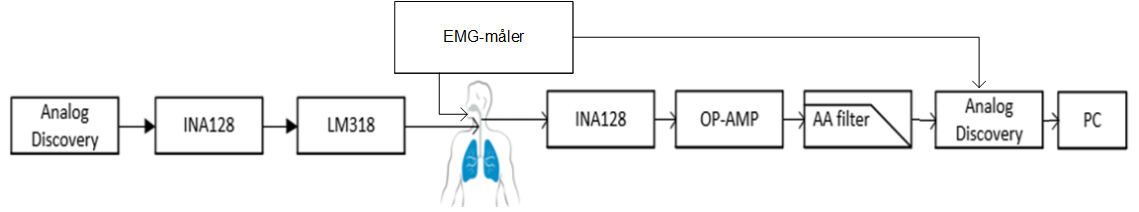
\includegraphics[width=\textwidth]
{Figure/Blokaede}}
\caption{Figuren viser de kommercielle komponenter, samt de enkelte komponenter, som skal designes for at realisere SRM.}
\label{fig:Blokaede}
\end{figure}

\subsection{Analog Discovery}

AD har i dette bachelorprojekt to formål. Den skal fungere som funktionsgenerator og som dataopsamlingsmodul. Figur \ref{fig:ADogINA128} viser disse to formål. Det ene formål er at funktionsgeneratoren genererer et AC signal med amplituden på 2 V og 20 kHz, som sendes til indgangen af instrumentationsforstærkeren INA128. Signalet bliver brugt til at generere en konstant strøm ud af operationsforstærkeren LM318N. Det andet formål er at AD modtager signal fra anti-aliaseringsfilteret.

\begin{figure}[H]
\centering
{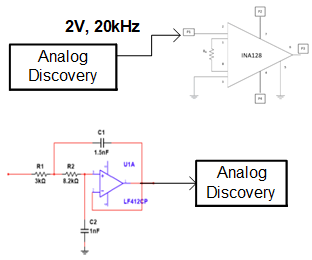
\includegraphics[width=10cm]
{Figure/ADogINA128}}
\caption{Figuren viser AD's funktioner i det samlede system. AD fungerer som funktionsgenerator og som dataopsamlingsmodul.}
\label{fig:ADogINA128}
\end{figure}

For at foretage korrekt dataopsamling af signaler fra analogt domæne til digitalt domæne, skal Shannons samplingsteori overholdes. Det vil sige at samplingsfrekvensen skal minimum være det dobbelte af den maksimale frekvenskomponent, Nyquist-frekvensen. Frekvenser større end Nyquist-frekvensen giver anledning til aliasering. Dette vil resultere i et fejlsignal. Derfor vælges der en samlingsfrekvens, som er væsentlig højere end den maksimale frekvenskomponent. 

Valg af dataopsamlingsmodul har også betydning for overgangen fra analogt domæne til digitalt domæne. Her konverteres de analoge værdier til de nærmeste digitale værdier. Konverteringen bestemmes af ADC'ens spændingsområde og opløsning. Forholdet i mellem spændingsområdet og opløsningen, udtrykkes LSB. LSB er et udtryk for den mindste detekterbare spændingsændring som ADC'en kan detektere. I henhold til AD's datablad, se \nameref{bilag15}, er denne opløsning på 14 bit. AD forsynes med en spænding på 10 V fra OP-AMP, som designes senere. Da man nu kender  spændingsområdet og opløsningen kan LSB bestemmes. LSB er beregnet til 0,48 mV. Der henvises til \nameref{bilag5}, for den fulde udregning af LSB.

Derfor er det besluttet at bruge AD, da den har følgende fordele:
\begin{itemize}
\item Den kan fungere som funktionsgenerator samtidig med, at den læser to signaler ind simultant
\item Den kan sample to signaler simultant med en samplingsfrekvens på 500 kHz
\item Den kan fungere som dataopsamlingsenhed
\end{itemize}



\subsection{Instrumentationsforstærker}

Instrumentationsforstærkeren i dette bachelorprojekt, har til formål at undertrykke støj fra måleobjekt og efterfølgende forstærke signalet, men også forstærke indgangssignalet fra AD's funktionsgenerator. Derfor anvendes i dette
projekt to instrumentationsforstærkere af typen INA128P. INA128P specifikationer kan læses i \nameref{bilag15}. INA128P giver mulighed for at forstærke signalet vha. kun en modstand. Fordelene ved anvendelse af instrumentationsforstærker, når det ønskes at måle elektrofysiologiske signaler er\cite{PeterJohansen2014}:
\begin{itemize}
\item 	Høj indgangsimpedans på ca. $10^{10} \Omega $
\item	Stor common mode rejection (CMR) på minimum 120dB
\item 	Differentielt input-single ended out (nødvendigt for at mindske $CM_{noise}$)
\end{itemize}



\textbf{Instrumentationsforstærker 1}

Den første INA128 benyttes til at forstærke signalet og undertrykke støj fra AD's funktionsgenerator. Det ønskes at forstærke de 2 V fra AD til 4 V. Det vil sige at gain er 2 og derfor kan R$_{G}$ modstanden beregnes til 50 k$\Omega$. Diagram over INA128 kan ses på figur \ref{fig:instrumentation1}. Udregning af R$_{G}$ og stykliste kan ses i \nameref{bilag5}.


\begin{figure}[H]
\centering
{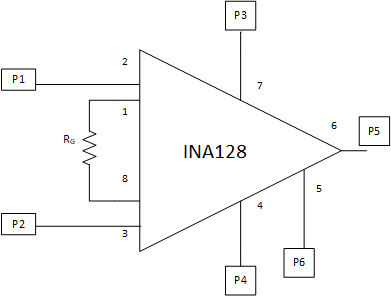
\includegraphics[width=10cm]
{Figure/instrumentation1}}
\caption{Figuren viser diagram for Instrumentationsforstærker 1 med tilhørende portnavne.}
\label{fig:instrumentation1}
\end{figure}



\pagebreak


\textbf{Instrumentationsforstærker 2}

Den anden INA128 anvendes til at forstærke elektrofysiologiske signaler fra måleobjektet og undertrykke commen mode støj. Det ønskes at INA128 forstærker med 100 gange, da det forventes at den målte spændingsforskel ligger i milli- og mikrovolt området\cite{PeterJohansen2014}. Diagram over INA128 kan ses på figur \ref{fig:instrumentation2}

\begin{figure}[H]
\centering
{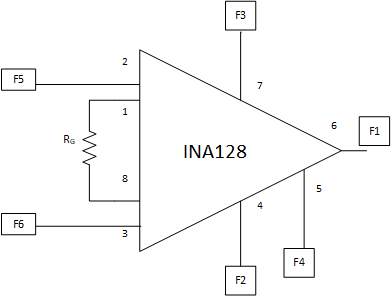
\includegraphics[width=10cm]
{Figure/instrumentation2}}
\caption{Figuren viser diagram for Instrumentationsforstærker 2 med tilhørende portnavne.}
\label{fig:instrumentation2}
\end{figure}

For at forstærkningen på 100 gange kan lade sig gøre, er det nødvendigt at slå op i databladet til INA128. Det kan konstateres at med en gain på 100, er det muligt at gå op til 100 kHz båndbredde, hvilken kan godkendes, der denne båndbredde ligger over anti-aliaseringsfilterets knækfrekvens på 25 kHz. Det er nu muligt at udregne størrelsen af R$_{G}$ modstanden. Denne størrelse er beregnet til at være 505 $\Omega$. Til en fremtidig modultest af INA128's gain på 100 gange, blev der designet en spændingsdeler til formålet. Diagram over spændingsdeleren kan ses på figur \ref{fig:spaedingdeler}. Udregning af R$_{G}$ og stykliste kan ses i \nameref{bilag5}.

\begin{figure}[H]
\centering
{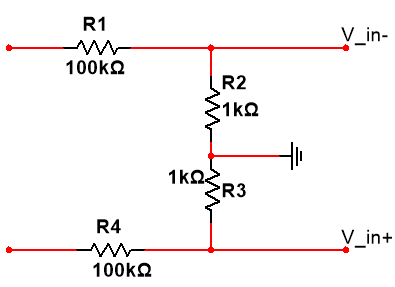
\includegraphics[width=8cm]
{Figure/spaedingdeler}}
\caption{Figuren viser diagram for spændingsdeleren.}
\label{fig:spaedingdeler}
\end{figure}

 
 
\subsection{Strømgenerator}
Strømgeneratoren i dette bachelorprojekt, har til formål at generere en strøm til måleobjektet gennem elektroderne. Dette er et krav for at kunne udføre en BI-måling på et måleobjekt\cite{Brantlov2017}. Diagram over strømgeneratoren kan ses på figur \ref{fig:StromgeneratorLM318}.

\begin{figure}[H]
\centering
{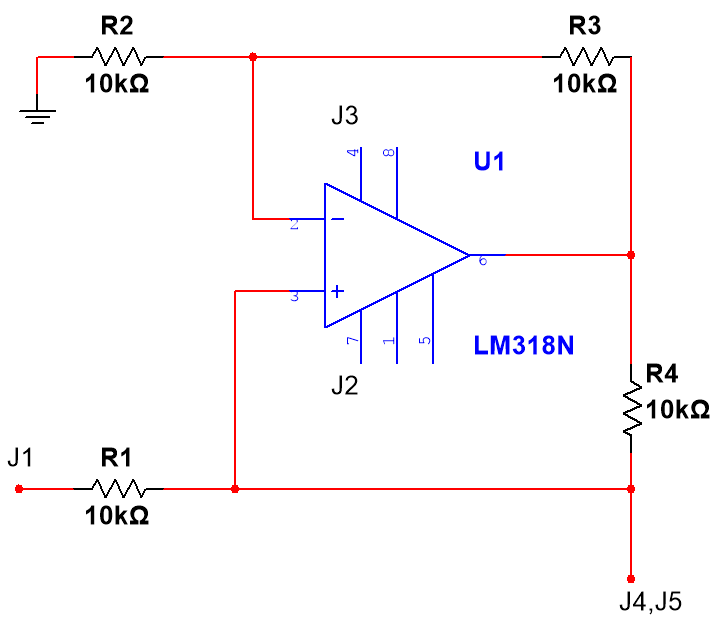
\includegraphics[width=10cm]
{Figure/StromgeneratorLM318}}
\caption{Figuren viser diagram for strømgenerator med tilhørende portnavne.}
\label{fig:StromgeneratorLM318}
\end{figure}

Strømgeneratoren også kaldet VCCS er designet efter en basis Howland pumpe. Ved udvælgelse af operationsforstærker kigges der på slewrate som skal overholdes. For at udregne slewrate bruges 20 kHz og 4 V. Slewrate udregnes til 0,503 V/$\mu$s. Her vælges operationsforstærkeren LM318, da den oplyses i databladet til at have en slewrate på 70 V/$\mu$s og den består kun en operationsforstærker, se \nameref{bilag15}. Den forventet strøm blev udregnet til 283 $\mu$A. Udregning af Howland pumpen, slew rate og stykliste kan læses i \nameref{bilag5}.

\pagebreak

\subsection{OP-AMP}
OP-AMP i dette bachelorprojekt har til formål at forstærke output signalet fra Instrumentationsforstærker 2. Der er valgt at benytte en ikke-inverterende operationsforstærker. Det ønskes at den forstærker op for at udnytte AD inputområde, som ligger mellem $\pm$25 V. Diagram over OP-AMP kan ses på figur \ref{fig:IkkeInviterendeOpAmp}.



\begin{figure}[H]
\centering
{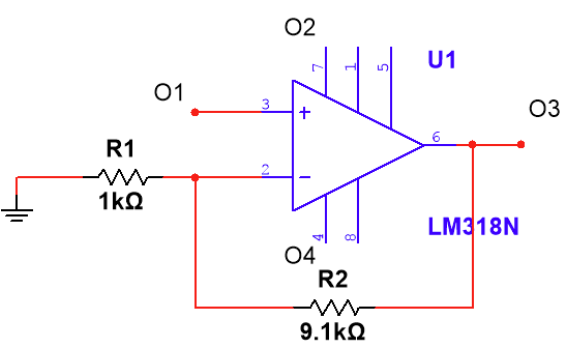
\includegraphics[width=10cm]
{Figure/IkkeInviterendeOpAmp}}
\caption{Figuren viser diagram for OP-AMP med tilhørende portnavne.}
\label{fig:IkkeInviterendeOpAmp}
\end{figure}

Signalet forstærkes op til 10 V, hvor gain udregnes ud fra forholdet mellem to modstande i OP-AMP kredsløbet. Den ene modstand sættes til 1 k$\Omega$ og den anden modstand udregnes til 9 k$\Omega$. Slew rate udregnes til 1,257 V/$\mu$s. Igen vælges operationsforstærkeren LM318, da den oplyses i databladet til at have en slewrate på 70 V/$\mu$s og den består kun en operationsforstærker. Udregninger af gain modstande og slew rate samt stykliste findes i \nameref{bilag5}.


\subsection{AA filter}

AA filter i dette bachelorprojekt, har til formål at dæmpe signalet over den halve samplingfrekvens (Nyquist frekvensen). Samplingfrekvensen vælges til 500 kHz, derfor bliver Nyquist frekvensen 250 kHz. AD er en 14 bit ADC, hvilket stiller krav om at signalet ved 250 kHz skal være dæmpet under $1/2*LSB$, som i dB svarer til en dæmpning på $20log*2^{15}=90dB$. På baggrund af spektrumanalysen i modultesten som står i \nameref{bilag6}, er det målte signal i forvejen dæmpet ca. 75 dB. Derfor ønskes at AA filter leverer en yderligere dæmpning med 20 dB. Dette anti-aliseringsfilter designes så det tillader passering af frekvenser, der er mindre en Nyquist frekvensen og dæmper frekvenser som er højere. Den yderligere dæmpning kan lade sig gøre med et første ordens filter, da det dæmper med 20 dB pr. dekade. Dog vælges i stedet et 2. ordens filter, der dæmper 40 dB pr. dekade. Det skal bemærkes at dette filter ikke påvirker det amplitude moduleret signal (synk) som ligger ved 20 kHz, da det stadig er indenfor for passbåndet og derfor ikke blive filteret væk. Diagram over AA filter kan ses på figur \ref{fig:aafilterdiagram}.

\begin{figure}[H]
\centering
{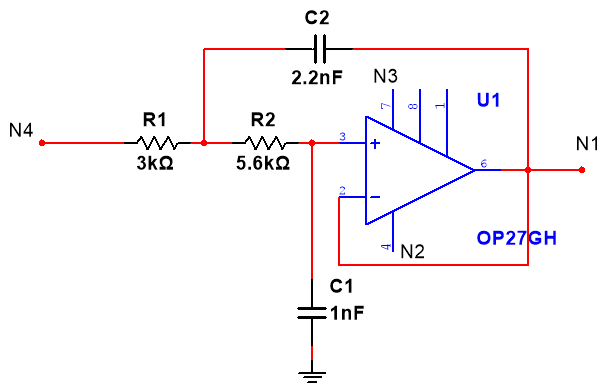
\includegraphics[width=10cm]
{Figure/aafilterdiagram}}
\caption{Figuren viser diagram for AA filter med tilhørende portnavne.}
\label{fig:aafilterdiagram}
\end{figure}


AA filteret designes derfor med følgende specifikationer:
\begin{itemize}
\item Aktivt lavpasfilter
\item 2. ordens Butterworth
\item Sallen key
\item Knækfrekvens = 25 kHz
\end{itemize}

På baggrund af overstående specifikationer er disse indtastet i programmet FilterPro. Dette resulterer i et design med komponent værdier, stykliste og diagram over filteret. 

Her foretages to yderligere udregninger slew rate og GBWP for at bestemme den korrekte operationsforstærker. Slew rate udregnes til 1,257 V/$\mu$s og GBWP til 2,5 MHz. Her vælges operationsforstærker OP27G, da der i databladet kan aflæses en slew rate på 2,8 V/$\mu$s og GBWP på 8 MHz. Hvilket stemmer fint overens med de udregnet værdier. Derudover er OP27G kendt fra tidligere semesterprojekt, hvor denne også skulle fungere som et lavpasfilter. Udregningerne for AA filter, bodeplot samt stykliste kan læses i \nameref{bilag5}.

\pagebreak

\section{Software}

Dette afsnit omhandler designet af softwaren, som anvendes til at håndtere AD, dataopsamling, analysering og visning af BI- og EMG-signaler. Denne designprocess har til formål at præsentere designede funktioner  i Matlab. Senere implementeres disse funktioner i Matlab.


\subsection{Funktioner}
Softwaren indeholder en række funktioner. Funktionerne har bestemte opgaver, hvilke funktionsnavnene afspejler af. I tabel \ref{tab:funktioner} er der vist tre funktioner med navn, type og en beskrivelse af hver funktion. Alle funktionerne og deres beskrivelse står beskrevet i \nameref{bilag5}. 

\begin{table}[H]

\begin{tabularx}{\textwidth}{l l X}
     Navn	&	Type		&	Beskrivelse \\ \midrule
     Generate\_SineWave	&	Funktion	&	Funktionen opretter forbindelse til Analog Discovery, tilføjer funktionsgeneratoren samt dens indstillinger, amplitude 2 V og frekvens 20 kHz.\\   \addlinespace[2mm]
     Read\_Measurements	&	Funktion	&	Funktionen tilføjder de to analog input som bruges til måling af BI og EMG. Derudover sættes samplingfrekvensen til 500 kHz og at en måling skal vare 10 sekunder.\\   \addlinespace[2mm]
     Process\_Measurements	&	Funktion	&	Her bliver der foretaget envelope af BI målingen. Dette sker ved at dobbeltensrette BI-signalet og lavpasfiltrere det ved 500 Hz.   \\   \addlinespace[2mm]
     \bottomrule                                                                                                                   
    \end{tabularx}
    \caption {Tabellen viser beskrivelse af tre funktioner der er designet for SRM's software del.}
    \label{tab:funktioner}
	
\end{table}

Udover funktioneres beskrivelse er der også en beskrivelse af oprettelsen af attributterne for hver funktion. Attributterne repræsenterer bl.a. de målte signaler og analyseringen af disse. I tabel \ref{tab:SWinputoutput} er der vist tre funktioners input og output. Alle funktionerne og deres input/output står nærmere beskrevet i \nameref{bilag5}.


\begin{table}[H]
\center
\begin{tabularx}{\linewidth}{l  X  X}
     \textbf{Funktion}	&	\textbf{Input}		&	\textbf{Output} \\ \midrule
     Generate\_SineWave   	&		&	handles.GS\\   \addlinespace[2mm]\hline\addlinespace[2mm]
Read\_Measurements	&	handles.GS	&	handles.BI\\   \addlinespace[2mm]
			    &		&	handles.EMG\\   \addlinespace[2mm]
			    &		&	handles.timestamps\\   \addlinespace[2mm]\hline\addlinespace[2mm]
			    Process\_Measurements    &	handles.BI	&	handles.locs\_synk\\   \addlinespace[2mm]
						&	handles.EMG	&	handles.BIsignal\\   \addlinespace[2mm]
						&	handles.timestamps	&	handles.EMGsignal\\   \addlinespace[2mm]
						&	& handles.TID	\\   \addlinespace[2mm]\hline\addlinespace[2mm]
						 \bottomrule                                                                                                                   
    \end{tabularx}
    \caption {Tabellen viser tre funktioner med deres input og output parametre.}
    \label{tab:SWinputoutput}
	
\end{table}

På figur \ref{fig:designSWenvelope} er der vist logikken bag behandlingen af BI signalet. Da signalet nu ligger i det digitale domæne, er det nu muligt at arbejde videre med dette BI signal vha. digitale værktøjer såsom filtrering. I denne behandling af BI signalet sker der flere ting i en bestemt rækkefølge. Først behandles signalet vha. envelope, ved at dobbelt ensrette og lavpas filtrere BI-signalet (knækfrekvens på 500 Hz og dæmpning på 40 dB pr. dekade). Dette resulterer i en konstant amplitude og samtidig flyttet BI signalet ned fra den 20 kHz bærebølge. Efterfølgende bliver BI signalet detrended, hvilket gør at BI signalet nu ligger pænt vandret over den best fittet linje i BI signalet. Dette giver mulighed for en nemmere analysering af BI-signalet. 

Da BI-signalet er samplet med 500 kHz, bliver det også downsamplet, da det giver en meget mindre mængde data at analysere og arbejde videre med. Derudover bliver BI signalet smooth, for at få fremhæve synket. Til slut findes der "peaks" (BI-signalets bakke dale), som kan bruges til at tælle antal synk i BI-signalet. Resultatet af denne logik er et pænt BI signal som vises på en graf og de fundne antal synk i BI-signalet. 

\begin{figure}[H]
\centering
{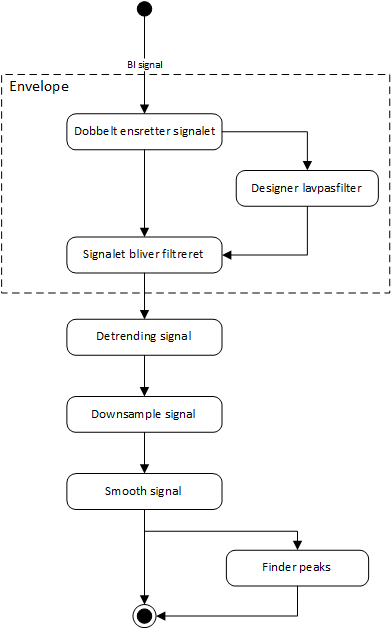
\includegraphics[width=10cm]
{Figure/designSWenvelope}}
\caption{Figuren viser et UML-aktivitetsdiagram over den interne logik i funktionen \textit{Process\_Measurements}, hvor BI-signalet bliver behandlet. }
\label{fig:designSWenvelope}
\end{figure}


\subsection{Sekvens Diagram}

Programmet startes ved at åbne m-filen Synkerefleksmonitor. Sundhedspersonalet kan herfra vælge at igangsætte en måling ved at trykke knappen \textit{"Btn\_Start\_Measurements"}. Gemme målingerne ved knappen \textit{"Btn\_Save\_Measurements"} og hente tidligere målinger via knappen \textit{"Btn\_Load\_Measurements"}. Disse knapper, samt resten af koden, kan vises i et sekvensdiagram med deres rækkefølge af kodeeksekvering. Sekvensdiagrammet kan ses på figur \ref{Fig:SekevensDiagram}.


\begin{figure}[H]
\centering
{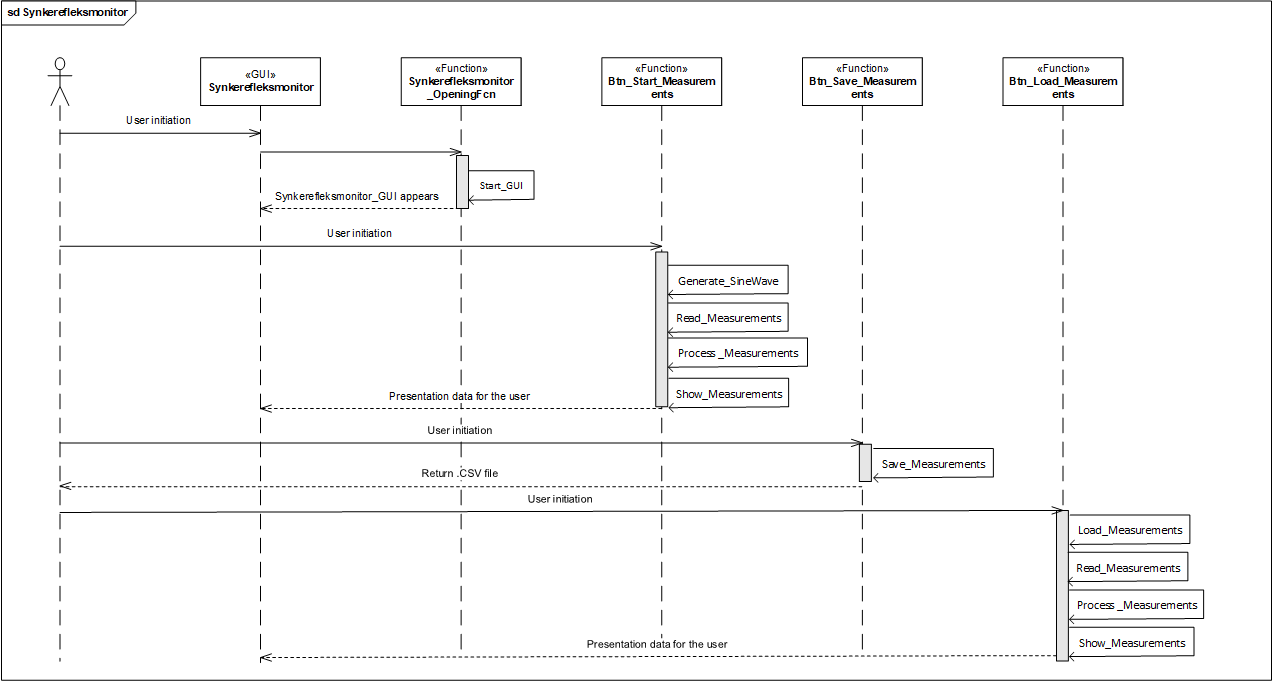
\includegraphics[width=\linewidth]
{Figure/SekevensDiagram}}
\caption{Figuren viser sekvensen af programmets kode}
\label{Fig:SekevensDiagram}
\end{figure} 


\subsection{GUI}

Softwaren til SRM består også af en GUI hvor sundhedspersonalet interagere med. På figur \ref{Fig:designGUI} kan GUI'en ses. Her har sundhedspersonalet mulighed for at foretage, gemme, og hente en tidligere måling. Designet af GUI er holdt meget simple og kræver ikke nogen yderligere introduktion af funktionaliteten, før programmet kan bruges. 

Der har også været i designfasen, fokus på feedback fra systemet til bruger. Da en måling fylder meget vil dette også tage tid at gemme, men under denne proces bliver der informeret, mens der gemmes og når CSV-filen er oprettet og gemt på computeren. En detaljeret beskrivelse af alle GUI'ens funktionaliteter kan ses i \nameref{bilag5}.


\begin{figure}[H]
\centering
{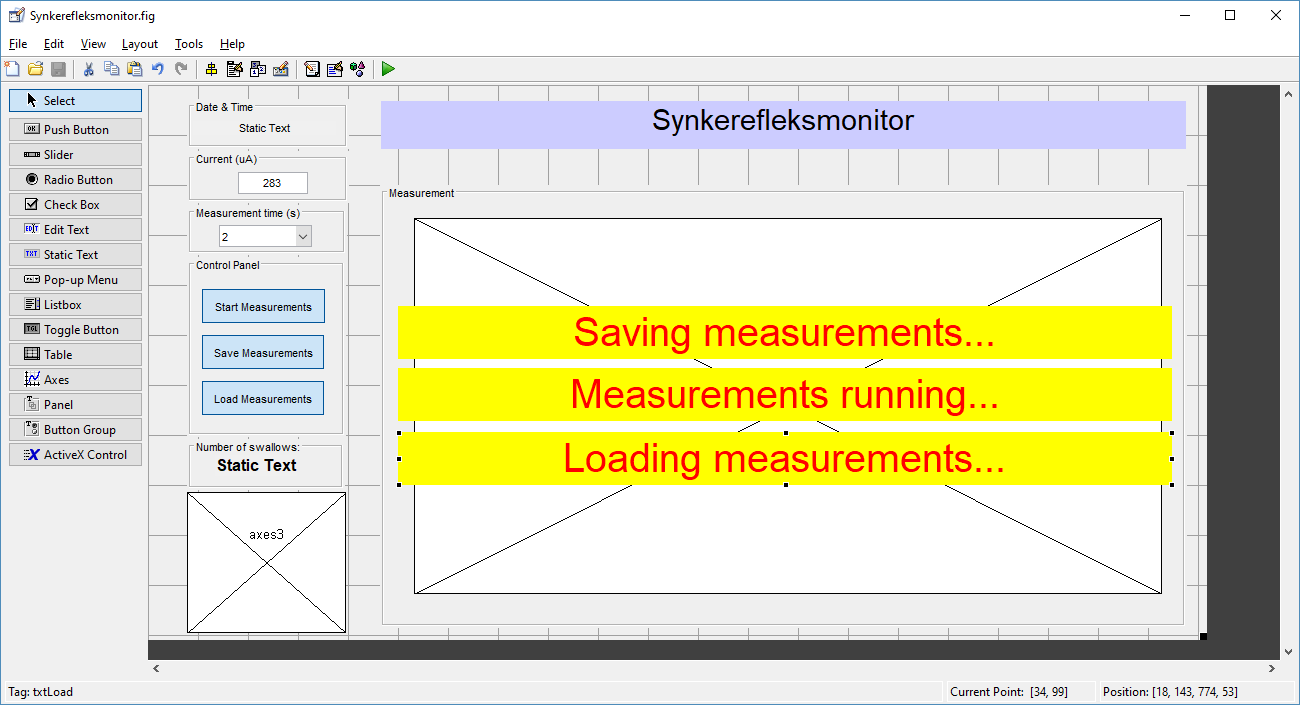
\includegraphics[width=14cm]
{Figure/designGUI}}
\caption{Figuren viser designet af GUI til SRM.}
\label{Fig:designGUI}
\end{figure} 